\section{Matrices de conexiones modulares}
\sectionmark{Matrices de conexiones}

Si hay algo que caracteriza a los sintetizadores de EMS es la forma en la que se se realizan las conexiones entre los módulos (Fig. \ref{fig:sinte_modular}). No es necesario el uso de un solo cable para ordenar las entradas y salidas. En lugar de tener un único conector para cada salida o entrada, Synthi 100 tiene dos matrices bidimiensionales cuyas ordenadas representan a las salidas y las abcisas las entradas de todos los módulos. Cada uno de sus nodos representa, por tanto, una conexión posible, a modo de coordenada. Las matrices del Synthi 100 del GME de Cuenca tienen unas dimensiones de 66 columnas por 60 filas, si bien algunas de estas no tienen ninguna conexión en este momento. En la matriz de \textit{Audio Control} existen 59 filas y 64 columnas, haciendo un total de 3776 conexiones individuales posibles. La de \textit{Voltage Control}, asimismo, 56 filas por 65 columnas, con un total de 3640 individuales posibles.

La conexión se realiza por medio de unas clavijas que, al introducirse en la conexión hembra, cierran el circuito. La limpieza visual de las conexiones es indiscutible respecto al paradigma del sintetizador modular por cables, especialmente cuando el número de conexiones es significativa; es muy fácil de reflejar en tablas sobre papel (Fig. \ref{fig:dope_sheet_GME}), incluso es posible escribirlo con coordenadas numéricas, ya que cada salida o entrada tiene un número único asignado (Fig. \ref{fig:patchbay_audio_vista_gral}).

\begin{figure}
	\centering
	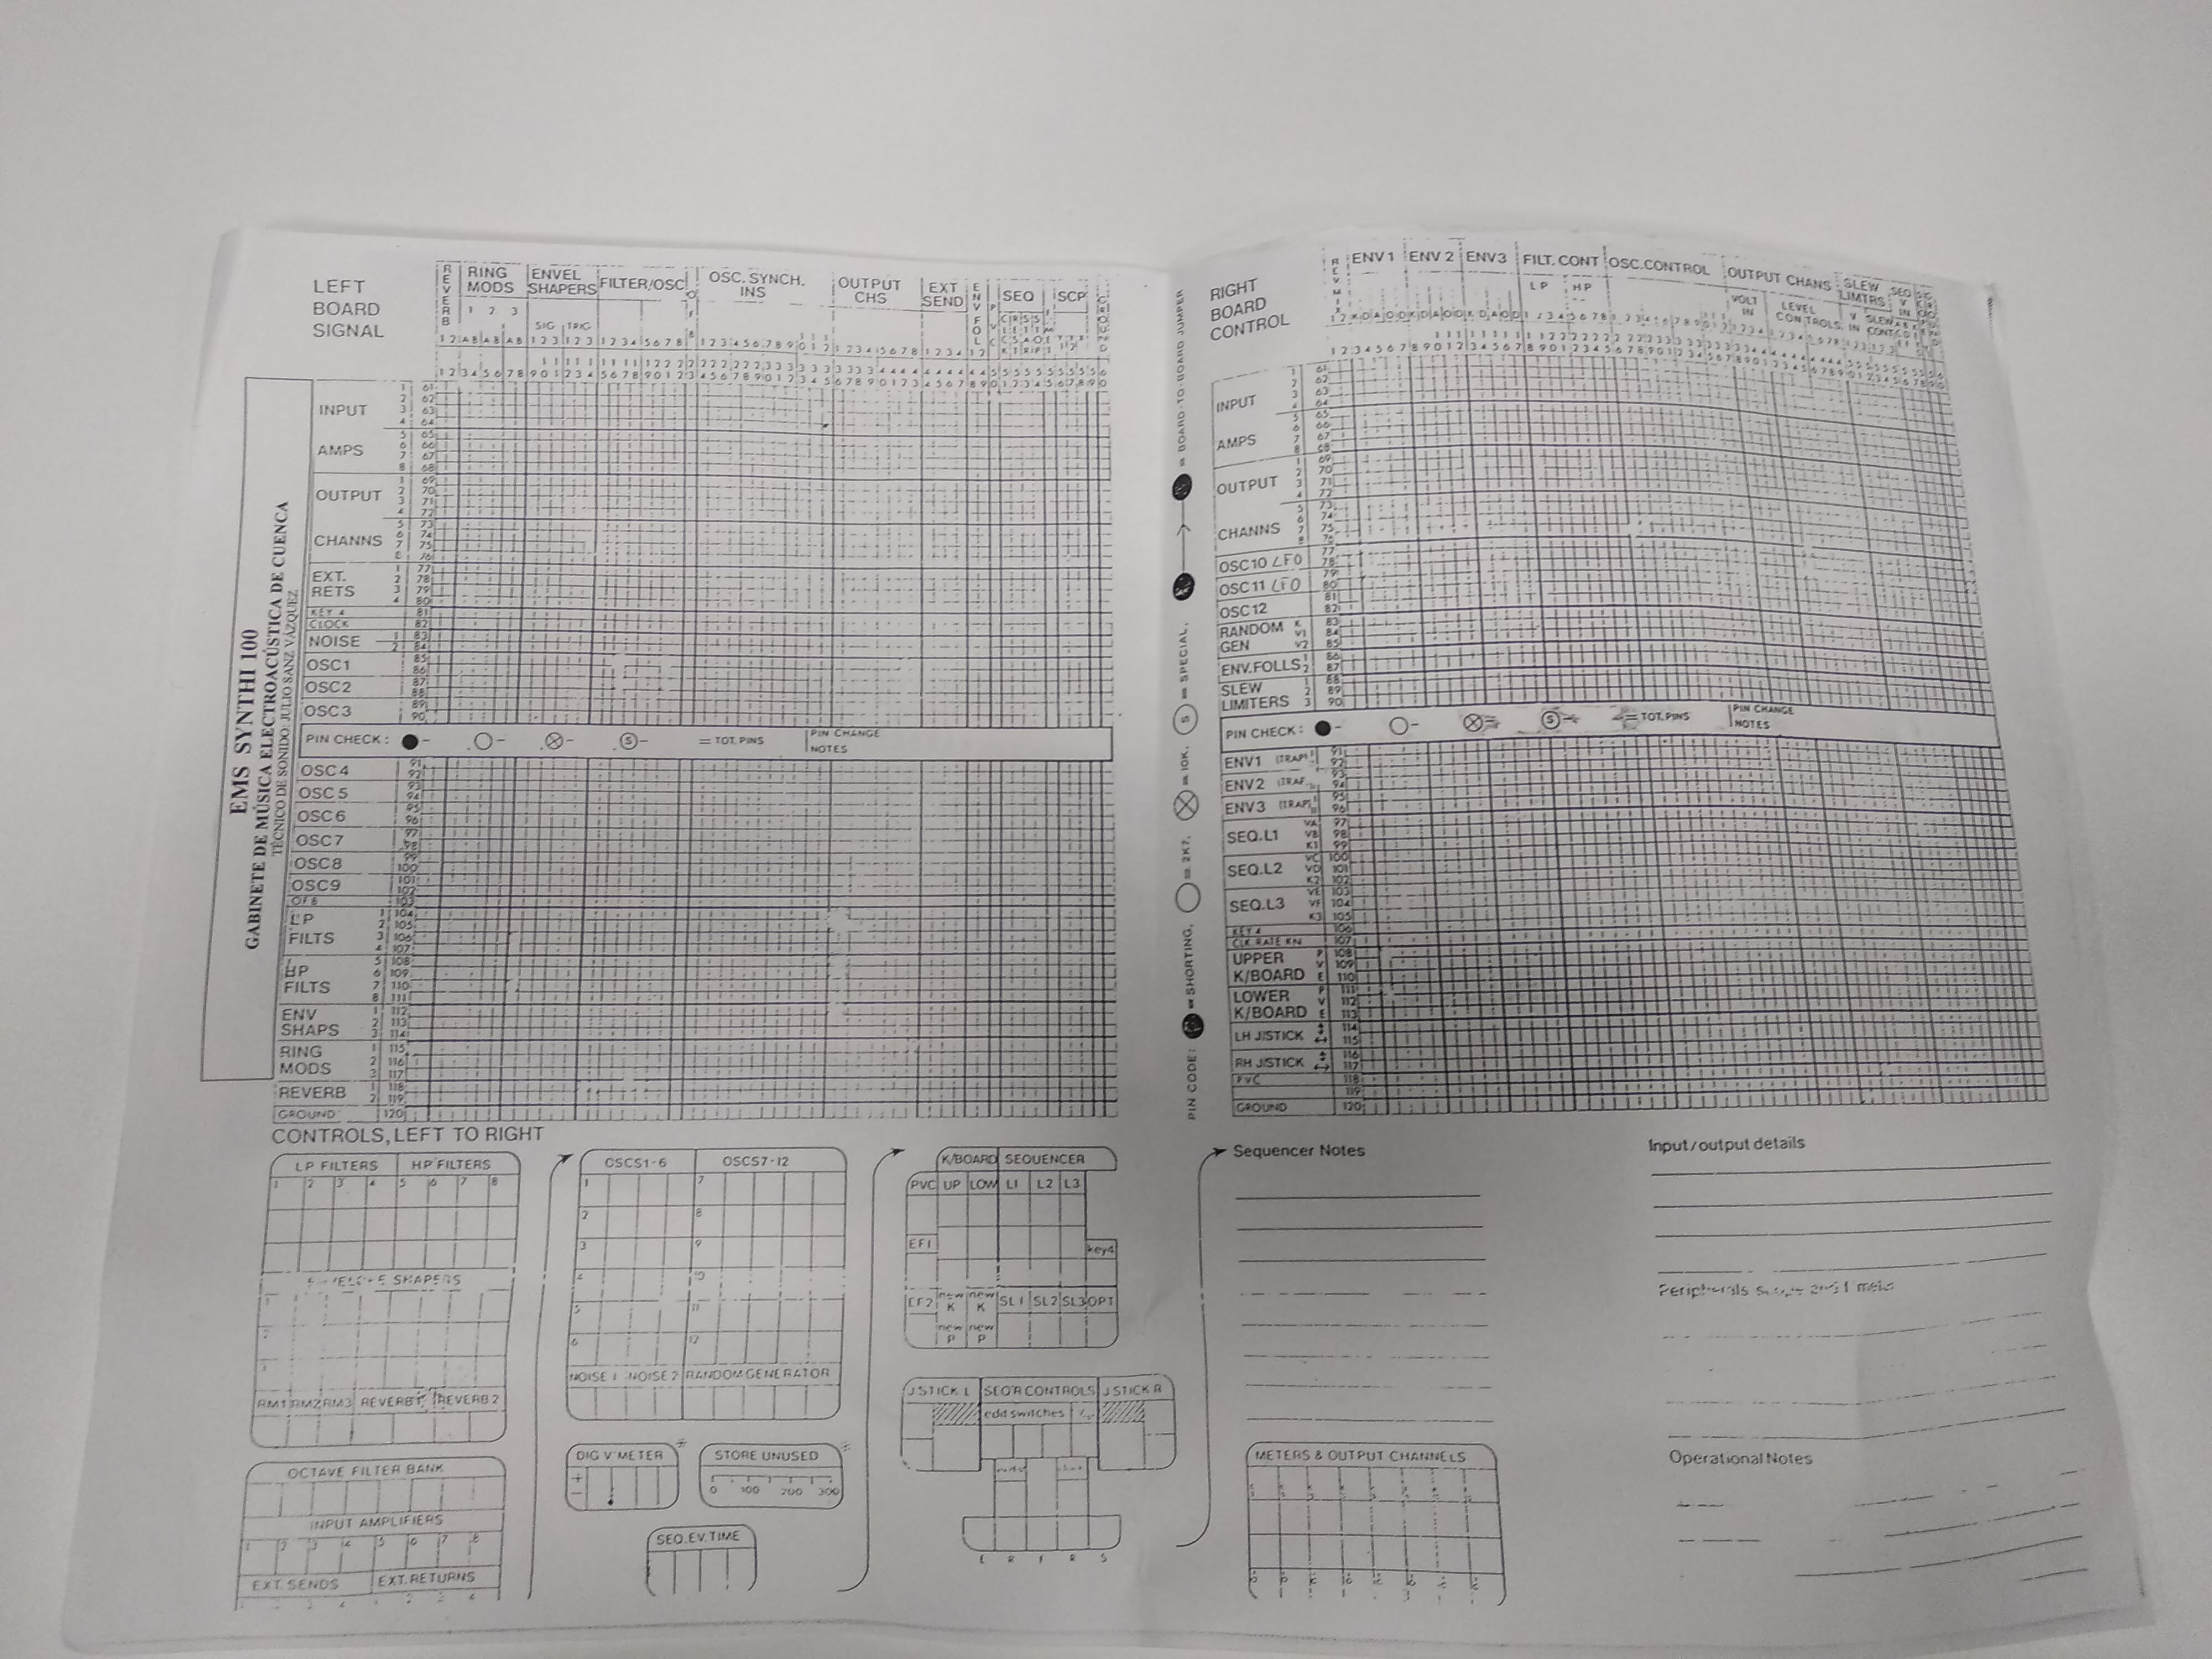
\includegraphics[width=0.7\textwidth]{images/dope_sheet_GME}
	\caption[\textit{Dope Sheet} conservado en el GME]{\textit{Dope Sheet} conservado en el GME. Hoja en la que el compositor o técnico encargado del GME tomaba nota esquemática de todas las conexiones y de los valores de ciertos módulos con el fin de poder repetirlos en el futuro}
	\label{fig:dope_sheet_GME}
\end{figure}

\begin{figure}
	\centering
	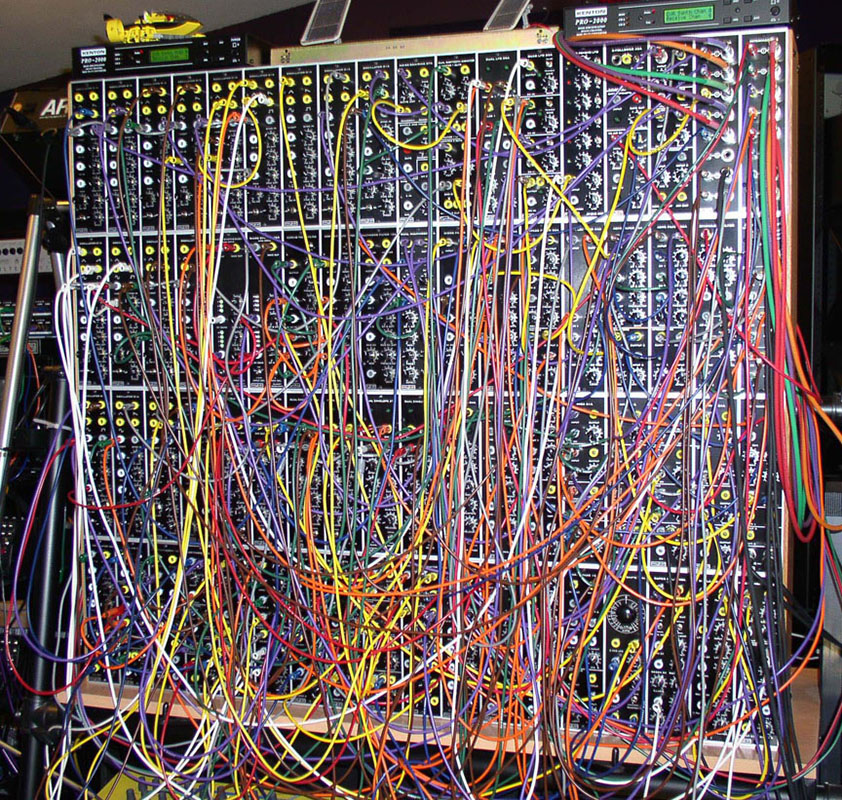
\includegraphics[width=0.7\textwidth]{images/sinte_modular}
	\caption[Tipico cableado de un sintetizador modular]{Tipico cableado de un sintetizador modular. Las salidas de un módulo se conectan por medio de cables con las entradas de otros módulos. La configuración del cableado determina en parte los resultados sonoros del conjunto. A pesar de lo intuitivo del sistema y su extendido uso, la complejidad de los cruces de cables le confieren una apariencia de gran complejidad.}
	\label{fig:sinte_modular}
\end{figure}

\subsection{\textit{Audio Control}}


\subsection{\textit{Voltage Control}}

\begin{figure}
	\centering
	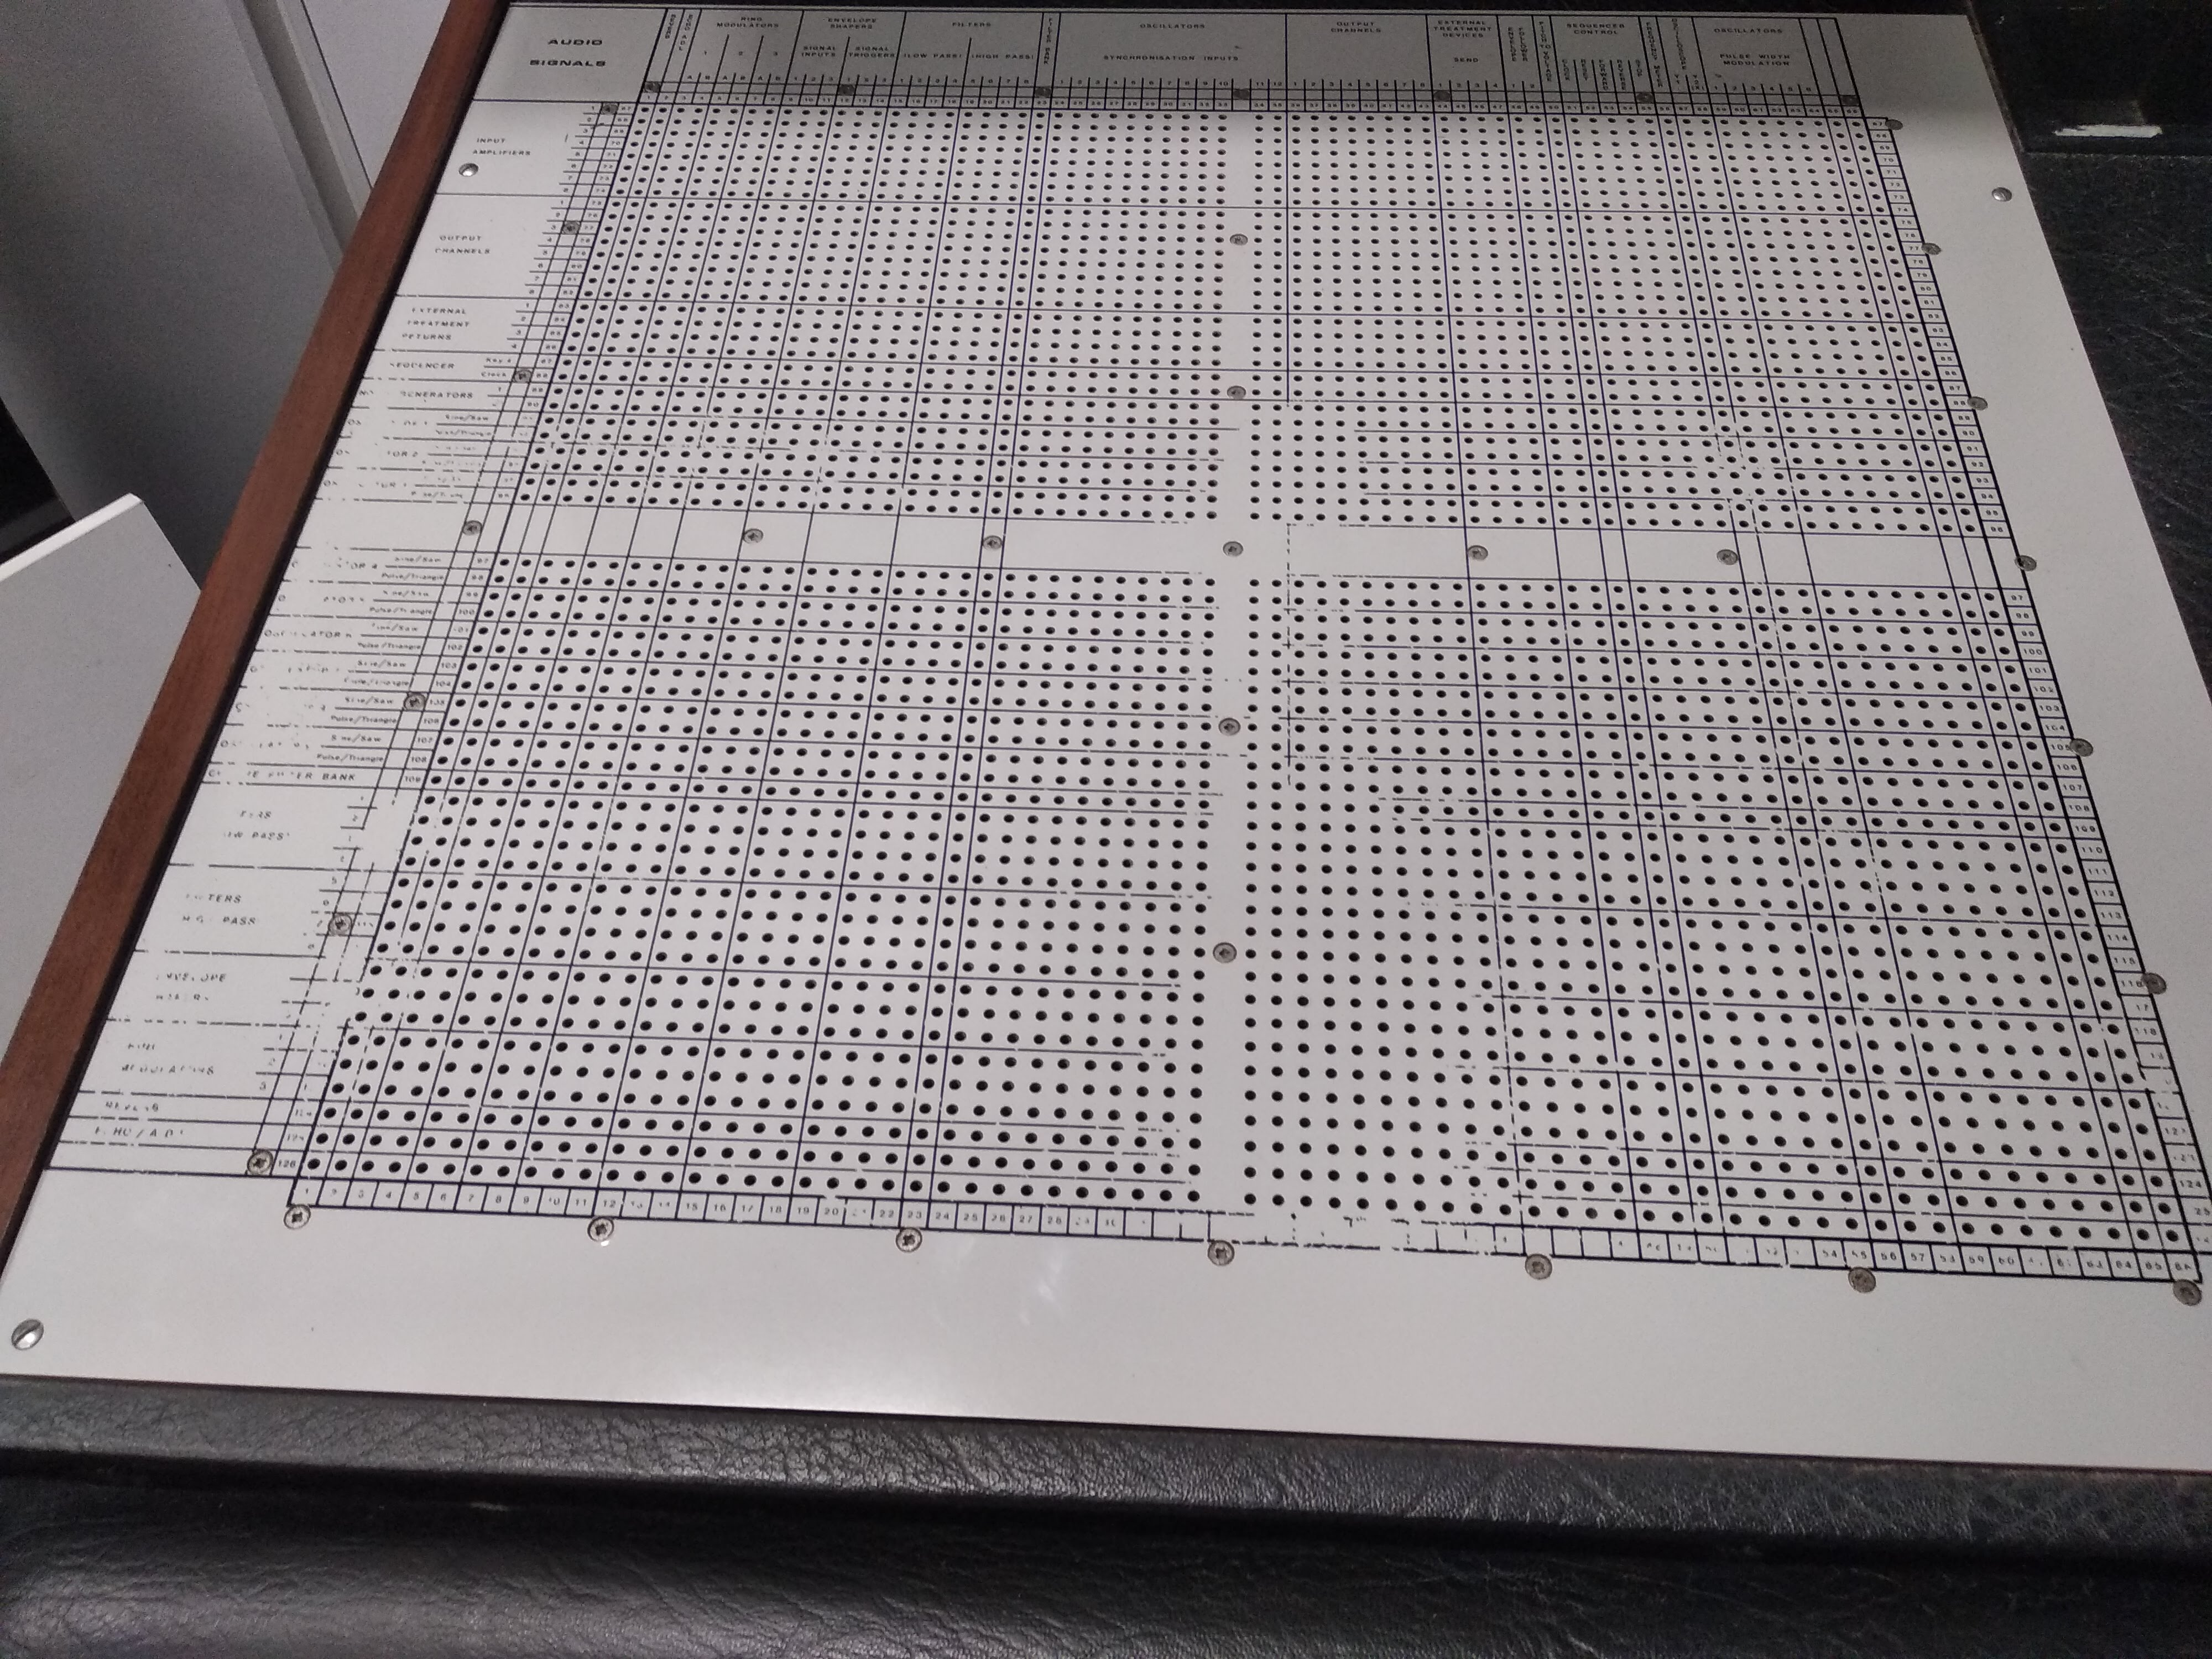
\includegraphics[width=0.8\textwidth]{images/patchbay_audio_vista_gral}
	\caption[Matriz \textit{Audio Control} del Synthi 100 del GME]{Matriz \textit{Audio Control} del Synthi 100 del GME. En vertical están ordendas todas las salidas de audio de todos los módulos, mientras que en horizontal se encuentran todas las entradas. Cada nodo representa una conexión única de una entrada con una salida. Los espacios que cruzan por el centro, así como los diversos grosores de las líneas dibujadas, ayudan visualmente a situar el nodo en las coordenadas deseadas. En la fotografía se observa sensiblemente el deterioro de los textos impresos debidos al uso continuado.}
	\label{fig:patchbay_audio_vista_gral}
\end{figure}

\subsection{Implementación en \appName}

\subsubsection[]{Administración de conexiones}
ORDEN DE EJECUCIÓN: InFeedback.ar
UNA CONEXIÓN = UN SYNTH

\subsubsection[]{Diseño de las matrices en \textit{GUI}}